\documentclass[sn-vancouver-num]{sn-jnl}
\usepackage[utf8]{inputenc}
\usepackage[T1]{fontenc}
\usepackage{makecell}
\usepackage{xcolor}
\usepackage{hyperref}
\hypersetup{
    colorlinks=true,
    linkcolor=blue,
    citecolor=blue,
    urlcolor=blue
}
\usepackage{caption}
\usepackage{float}
\usepackage{parskip}
\usepackage{enumitem}
\usepackage{graphicx}
\usepackage{booktabs}
\usepackage{longtable}
\usepackage{geometry}
\usepackage{amsmath}
\usepackage{tabularx}
\newcolumntype{Y}{>{\raggedright\arraybackslash}X}
\makeatletter
\renewcommand{\Authorfont}{\reset@font\fontsize{10bp}{12bp}\selectfont\boldmath\titraggedcenter}
\renewcommand{\addressfont}{\reset@font\fontsize{8.5bp}{10.5bp}\selectfont\titraggedcenter}
\let\PrismOriginalPrintAbstract\printabstract
\renewcommand{\printabstract}{\newpage\PrismOriginalPrintAbstract}
\makeatother

\begin{document}

\title{A Closed-Loop Framework for Knowledge-Based Causal Model Refinement Using Process Mining and Human--AI Governance}

\author*[1]{\fnm{Eduardo} \sur{Illueca-Fernandez}}
\author[1,2]{\fnm{Kaile} \sur{Chen}}
\author[1,3,4,5]{\fnm{Fernando} \sur{Seoane}}
\author*[1,2,3]{\fnm{Farhad} \sur{Abtahi}}\email{farhad.abtahi@ki.se}


\affil[1]{\orgdiv{Department of Clinical Science, Intervention and Technology}, \orgname{Karolinska Institutet}, \city{Stockholm}, \postcode{17177}, \country{Sweden}}
\affil[2]{\orgdiv{Department of Biomedical Engineering and Health Systems}, \orgname{KTH Royal Institute of Technology}, \city{Huddinge}, \postcode{14157}, \country{Sweden}}
\affil[3]{\orgdiv{Department of Clinical Physiology}, \orgname{Karolinska University Hospital}, \city{Stockholm}, \postcode{17176}, \country{Sweden}}
\affil[4]{\orgdiv{Department of Medical Technology}, \orgname{Karolinska University Hospital}, \city{Stockholm}, \postcode{17176}, \country{Sweden}}
\affil[5]{\orgdiv{Department of Textile Technology}, \orgname{University of Borås}, \city{Borås}, \postcode{50190}, \country{Sweden}}


\abstract{
\textbf{Background:} Directed acyclic graphs (DAGs) are fundamental to causal inference in epidemiology, yet their construction typically relies on expert opinion without systematic empirical challenge. When causal structures are uncertain, as in chronic disease settings with competing risks and complex temporal dynamics, DAG misspecification can bias effect estimates regardless of analytical sophistication. We present a closed-loop framework that treats knowledge-based DAGs as testable hypotheses, iteratively refined through process mining evidence and governed human–AI collaboration.

\textbf{Methods:} The framework comprises four phases: (1) knowledge-driven event log construction using LLM-assisted literature synthesis and expert input; (2) data-driven pattern discovery through process mining of longitudinal event sequences; (3) structured DAG refinement through systematic comparison of empirical patterns against the knowledge-based DAG, with human expert adjudication of each proposed change; and (4) DAG-guided statistical model selection and assessment. We operationalised the framework through an open-source interactive tool, and demonstrated its performance using synthetic data calibrated to a published cohort of 294,734 individuals (Stockholm CREAtinine Measurements project) comparing proton pump inhibitor (PPI) and histamine-2 receptor blocker (H2B) users.

\textbf{Results:} In a synthetic tutorial dataset calibrated to published SCREAM cohort results, the workflow reproduced longitudinal patterns in which CKD progression preceded cardiovascular adverse events, illustrating how the framework would surface a candidate mediator pathway for expert adjudication. Formal mediation analysis would be required to test the mediator hypothesis. Competing mortality rates (CKD$\rightarrow$Death: 23.9\% PPI vs 17.9\% H2B; CVAE$\rightarrow$Death: 47.0\% vs 37.9\%) illustrated how high mortality transitions would prompt expert review of competing-event handling in the analytical model. The AI tool recommended Fine--Gray competing-risk models, causal mediation analysis, and propensity-score balancing, all consistent with epidemiological best practice.

\textbf{Conclusions:} The closed-loop framework provides a governed, transparent, and reproducible approach for integrating AI assistance into causal inference workflows. By embedding empirical appraisal into DAG construction while preserving human authority over causal interpretation, the framework advances methodological discipline in real-world evidence generation.
}

\keywords{causal inference, directed acyclic graphs, process mining, human-AI collaboration, real-world evidence, disease trajectories, longitudinal data}

\maketitle
\newpage

\section{Introduction}
Epidemiological causal inference relies on accurately specifying causal relationships among variables \citep{vanderweele2019,pearl2010}. To infer causality from observational data, epidemiology employs regression-based adjustment, inverse probability weighting, and instrumental variable methods, guided by graphical representations of causal assumptions. Directed acyclic graphs (DAGs) encode these assumptions as nodes (variables) connected by directed edges (assumed causal effects) and guide the selection of statistical analyses that target the causal estimands of interest \citep{pearl2009,greenland1999,hernan2004}. A well-specified DAG ensures valid causal inference, while a mis-specified DAG can lead to biased estimates regardless of statistical sophistication \citep{digitale2022,lederer2019,tennant2021}. The challenge arises when causal structures are uncertain, a common scenario in chronic disease epidemiology where multiple interacting conditions, time-varying exposures, competing risks, and complex temporal dynamics create causal ambiguity  \citep{hernan2019,glymour2019}.

The need for methodological innovation is particularly acute in the era of real-world data (RWD) and real-world evidence (RWE). Healthcare systems generate vast longitudinal datasets through electronic health records (EHRs), administrative claims databases, disease registries, and patient-reported outcomes. While randomized controlled trials (RCTs) remain the gold standard for establishing efficacy under controlled conditions, real-world data provide essential complementary evidence on effectiveness, safety, long-term outcomes, and treatment patterns in diverse, unselected populations reflecting actual clinical practice  \citep{sherman2016}. However, the same characteristics that make RWD valuable also present distinct methodological challenges. Causal uncertainty increases with scale: when thousands of variables interact over years or decades, pre-specifying all causal relationships is impractical. Temporal complexity arises from irregular visit times, varying follow-up lengths, and missing episodes \citep{casey2016}. Competing risks and informative censoring mean that multiple outcomes may prevent observation of events of interest. Clinical heterogeneity and trajectory variation across diverse populations produce disease courses that aggregate statistics may obscure \citep{burns2022}.

Aligning with the classical roots of epidemiological investigation proposed by Dr. John Snow \citep{coleman2019causality}, causal inference is increasingly recognised as a falsifiable and iterative scientific process in which causal assumptions are continuously tested, refined, and assessed against real-world evidence \citep{ahsen2025}. This perspective helps bridge the persistent divide between theoretical epidemiology and empirical discovery, emphasizing that causal understanding emerges through a continuous dialogue between conceptual models and observational data. Initial causal assumptions, grounded in domain expertise and prior literature, are explicitly formulated as testable hypotheses using directed acyclic graphs (DAGs). Then, these hypotheses can be examined through process mining of longitudinal event sequences to uncover temporal and sequential patterns that either support or challenge the theoretical model \citep{vanderaalst2016}. These empirical patterns can be formally represented using directly-follows graphs (DFGs), which capture observed transitions between events in longitudinal data. In this framework, the DFG serves as an empirical counterpart to the knowledge-based DAG, enabling systematic comparison between hypothesized causal structures and observed temporal patterns. Discrepancies between the hypothesized and observed structures prompt systematic refinement based on biological plausibility, clinical insight, and mechanistic understanding. The refined models are subsequently assessed using appropriate statistical techniques, following the interactive process mining approach \citep{fernandez2020}. Through this iterative cycle of hypothesis testing, refinement, and assessment, the framework provides a transparent and reproducible approach for generating robust causal evidence while maintaining the methodological rigor of causal epidemiology.

This paper introduces a governed, closed-loop diagnostic workflow that integrates causal modelling, data-driven pattern discovery, and statistical model selection to iteratively challenge and refine pre-specified causal assumptions using real-world data, without performing causal discovery or replacing formal identification strategies. Specifically, it seeks to address these challenges systematically by treating RWD analysis as an iterative process rather than a one-time statistical application \citep{ibanez2019}. In this sense, the Tutorial Demonstration section uses synthetic data calibrated to published results for illustrative purposes only. This manuscript consolidates the iterative methodological development into a unified governed framework. Specifically, we (1) formalise the four-phase refinement loop with explicit human adjudication at each transition, (2) define the  role of process mining as diagnostic appraisal of causal assumptions rather than causal proof, (3) embed auditability and provenance tracking as design requirements, and (4) demonstrate the complete workflow through an illustrative worked example using synthetic data.

The rest of the paper is structured as follows. First, the framework is positioned in relation to emerging AI methods in the \textit{State of the Art}. Then, our four-phase methodology is described in the \textit{Methodology}, and the resulting evidence-refined DAG is presented in the \textit{Results} section. Last, the Discussion describes how our framework addresses key challenges in causal epidemiology, clarifies when it provides the greatest value, and establishes governance infrastructure for integrating agentic AI systems, while preserving interpretability, biological plausibility, and clinical validity.

\section{State of the Art}
Before the mathematical formalization of modern epidemiology and the release of powerful artificial intelligence models, Dr. John Snow established the foundational archetype for causal inference using real-world data during the 1854 London cholera outbreak \citep{dayal2023john}. Rather than accepting the dominant "miasma" hypothesis of his era, he systematically collected observational field data, mapping cholera mortality at the household level to uncover spatial and sequential patterns. By demonstrating that exposure to specific water sources strictly preceded disease trajectories and that removing the Broad Street pump handle halted the outbreak, Snow successfully succeed by considering causal assumptions as testable, falsifiable hypotheses.

Despite this long-standing paradigm of empirical falsification, modern workflows for specifying causal relationships have largely remained isolated from the data they intend to analyze. Traditional knowledge-based DAGs \citep{vanderweele2019,pearl2010,pearl2009,greenland1999,hernan2004} rely on literature review and expert opinion to manually construct causal graphs. While these approaches ensure clinical plausibility, they risk misspecification when causal structures are uncertain or complex \citep{digitale2022,tennant2021}. Tools such as DAGitty and ggdag support DAG construction and identification of adjustment sets, but do not provide mechanisms for empirical appraisal of the assumed structure. 

Automated causal discovery algorithms, including constraint-based methods (PC, FCI) and score-based methods (GES) \citep{glymour2019,chickering2002}, infer causal structures from conditional independence tests or statistical fit optimisation. However, these methods rely on strong assumptions (faithfulness, causal sufficiency) that are rarely satisfied in complex healthcare data, and their outputs often lack clinical interpretability \citep{pearl2009,glymour2019}. More recently, large language models have been explored for causal reasoning, with studies demonstrating that LLMs can generate plausible causal graphs from textual descriptions \citep{kiciman2023,meier2025}. While promising for hypothesis generation at scale, these approaches raise concerns about hallucination, citation accuracy, and the opacity of the reasoning process.

Process mining offers a complementary perspective by discovering temporal patterns directly from longitudinal event data \citep{vanderaalst2016}. Originally developed for business process optimisation, process mining has been increasingly applied to healthcare for pathway analysis \citep{mans2008,rebuge2012,rojas2016,munoz2022}, clinical trajectory characterisation \citep{fernandez2015,kurniati2016,williams2018}, and care quality assessment \citep{ibanez2019}. Interactive process mining \citep{fernandez2020} emphasises continuous human-in-the-loop engagement, and question-driven approaches \citep{rojas2017} centre analysis around expert-formulated research questions. However, existing process mining applications in healthcare typically focus on descriptive pathway analysis rather than causal inference, and lack systematic frameworks for translating discoveries into causal model refinements \citep{chen2023,montoya2025}. 

The closed-loop framework presented in this paper seeks to implement and automatize John Snow's philosophy by integrating knowledge-based DAG specification with empirical temporal pattern discovery through process mining, while embedding human-AI governance to maintain clinical validity. Unlike purely automated methods, it preserves expert authority over causal decisions; unlike purely knowledge-based approaches, it provides a systematic mechanism for empirical challenge and refinement. Table~\ref{tab:sota} summarises the different  approaches discussed in this section. 

\begin{table}[h]
\caption{Comparison of approaches for causal structure specification in epidemiology.}
\label{tab:sota}
\centering
\footnotesize
\setlength{\tabcolsep}{3.5pt}
\renewcommand{\arraystretch}{1.15}
\begin{tabularx}{\textwidth}{@{}>{\raggedright\arraybackslash}p{2.6cm}YYYYYY@{}}
\toprule
\textbf{Approach} & \textbf{Primary input} & \textbf{Method} & \textbf{Clinical integration} & \textbf{AI role} & \textbf{Human role} & \textbf{Best suited for} \\
\midrule
Knowledge-based DAGs \citep{greenland1999} & Literature and expertise & Manual graph construction & High & Minimal & Central & Well-understood mechanisms \\
Constraint-based algorithms (PC, FCI) \citep{chickering2002} & Conditional independence tests & Algorithmic structure learning & Low & Automated discovery & Limited & High-dimensional exploration \\
Score-based algorithms \citep{chickering2002} & Statistical model fit & Search and optimisation & Low & Automated model comparison & Limited & Candidate-graph comparison \\
Agentic AI \citep{chickering2002} & LLMs and knowledge bases & Automated causal reasoning & Moderate & Hypothesis generation & Oversight & Scalable hypothesis generation \\
\textbf{Closed-loop framework} & Domain knowledge and longitudinal data & Iterative, governed refinement & \textbf{High} & Checkpoint augmentation & \textbf{Central} & Complex and uncertain structures \\
\bottomrule
\end{tabularx}
\end{table}

\section{Methodology}
Our proposed closed-loop methodology integrates theory and evidence through a structured, iterative refinement process. The framework is intended to support the refinement and documentation of knowledge-based causal models using longitudinal observational patterns and expert review without replacing a formal identification strategy, domain knowledge, or sensitivity analysis. Knowledge guides discovery, discovery refines knowledge, and clinical oversight maintains validity throughout. The framework is naturally compatible with AI automated tasks while ensuring human oversight remains central. The contribution lies in defining the governance structure and methodological infrastructure that enables AI systems to integrate responsibly into causal inference workflows. Clear roles are defined for AI assistance (hypothesis generation, pattern recognition, structural comparison) while human authority over biological plausibility, clinical interpretation, and causal adjudication is preserved.

\subsection{The Four-Phase Methodology}
Figure~\ref{fig:fourphase} illustrates the four-phase closed-loop methodology. First, Phase 1 initiates with knowledge-driven DAG construction and event log structuring, where an LLM synthesises literature and information stored in a Retrieval-Augmented Generation (RAG) into a knowledge-based DAG, which then guides event log design. Then, Phase 2 applies process mining algorithms to the event log to discover temporal patterns and generate an empirical process model based on real-world data. Consequently, Phase 3 involves the generation of the evidence-refined DAG. In this phase, the LLMs analyze the discrepancies between the DAG and the empirical process model and propose changes. In this context, the human expert can decide which changes should be applied and which ones should be rejected, producing an evidence-refined DAG. The resulting artifact, termed the evidence-refined DAG, is a directed acyclic graph whose hypothesised relationships have been empirically appraised against — and have not been falsified by — observed temporal patterns, and which retains the formal properties required for causal inference. The term "refined" denotes this iterative empirical appraisal under expert oversight; it does not imply that the DAG is data-validated or that its causal edges are empirically proven. Because process mining is restricted to measured variables and to recorded events, the DAG remains a representation of expert-adjudicated causal assumptions subject to standard threats to causal inference, including unmeasured confounding. 

In consequence, it differs from the initial knowledge-based DAG in that its structure has been tested against real-world event sequences and refined based on that evidence. It differs from automated causal discovery outputs in that every structural change requires explicit human approval grounded in biological plausibility and mechanistic understanding. Finally, Phase 4 performs statistical model assessment, where AI uses the evidence-refined DAG to recommend suitable causal models for estimating causal effects, leaving the selection of the final model to the human expert.

\begin{figure}
  \centering
  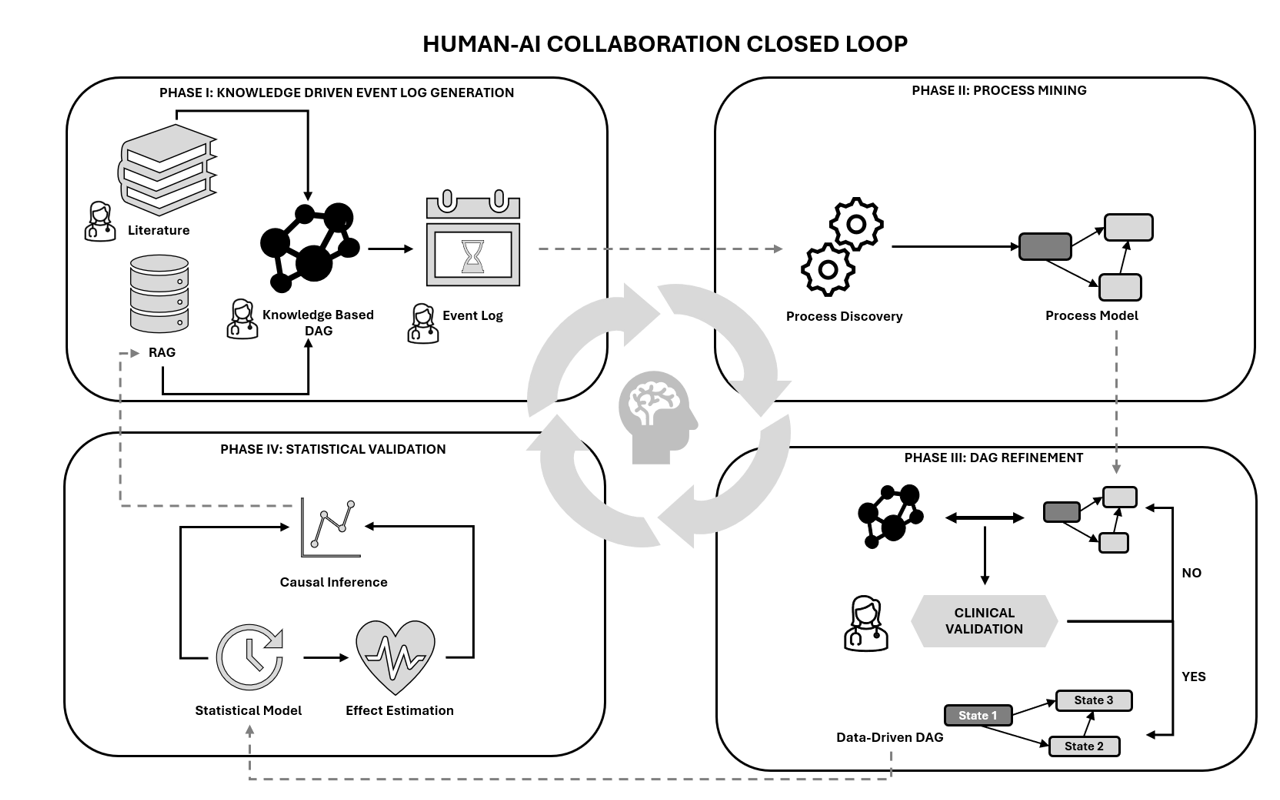
\includegraphics[width=\textwidth]{figures/figure1.png}
  \captionsetup{font=scriptsize}
  \caption{The four-phase closed-loop data-driven DAG methodology. Phase 1 (Knowledge) uses LLM-assisted literature synthesis and expert input to construct an initial knowledge-based DAG specifying exposures, outcomes, confounders, and mediators. Phase 2 (Discovery) applies process mining to real-world event logs, generating a directly-follows graph (DFG) of observed temporal transitions with associated frequencies and median times. Phase 3 (Refinement) systematically compares the DFG against the knowledge-based DAG; discrepancies generate candidate structural refinements that human experts accept or reject based on biological plausibility. Phase 4 (Validation) recommends statistical models informed by the refined DAG structure and provides executable analysis templates. The feedback loop from Phase 4 to Phase 1 enables iterative updating of the knowledge base. The framework is specifically designed for real-world healthcare data where causal structures are uncertain, temporal patterns are complex, and competing risks are common.}
  \label{fig:fourphase}
\end{figure}


Each phase of the closed-loop framework directly supports the rigorous specification and estimation of the target estimand. Phase 1 defines the theoretical causal contrasts by structuring the initial target trial protocol within the knowledge base. Phase 2 evaluates the feasibility of emulating these strategies by mapping the actual, real-world treatment pathways and event orderings. Phase 3 refines the estimand itself—for instance, by formally introducing competing events like death into the structural model, which dictates whether the target estimand should be conceptualized as a direct effect, a total effect, or a cumulative incidence. Finally, Phase 4 bridges the refined causal structure to the statistical estimator, ensuring the chosen models explicitly target the parameter defined by the target trial

This four-phase methodology integrates human expertise with AI capabilities in a closed-loop. Specifically, the RAG knowledge base used in Phase 1 is updated with the results collected from the causal inference done in Phase 4. This feedback loop constitutes a knowledge transfer mechanism in which the validated causal findings, refined DAG structures, and statistical results from Phase 4 are systematically incorporated back into the RAG knowledge base that informs Phase 1 of the next iteration. In concrete, the information added includes structural updates, including refined DAG architectures where causal assumptions have been retained, revised, deprioritized, or proposed for further evaluation; statistical evidence, such as precise causal effect estimates, p-values, and confidence intervals that quantify the strength of relationships; and expert knowledge, captured via decision logs that document the researcher's justification for model adjustments. 

In the presented framework, this transfer is operationalised through the client-side knowledge base: researchers can add their Phase 4 outputs, including model results, decision logs, and refined DAG exports, as new documents in the RAG system, ensuring that subsequent hypothesis generation is grounded not only in the published literature but also in the empirical findings of prior analytical cycles. This cumulative learning mechanism transforms the framework from a single-pass analytical pipeline into a genuinely iterative research programme, where each cycle produces both causal effect estimates and enriched domain knowledge that sharpens the next cycle's starting assumptions. Table~\ref{tab:phases} outlines the role, inputs, and outputs of each phase, research opportunities for AI enhancement, and critical limitations. 

\begin{table}[h]
\caption{Four-phase closed-loop methodology and governance roles.}
\label{tab:phases}
\centering
\scriptsize
\setlength{\tabcolsep}{4pt}
\renewcommand{\arraystretch}{1.18}
\begin{tabularx}{\textwidth}{@{}>{\raggedright\arraybackslash}p{2.4cm}YYYY@{}}
\toprule
\textbf{Phase} & \textbf{Current practice} & \textbf{AI enhancement opportunity} & \textbf{Key limitation} & \textbf{Human responsibility} \\
\midrule
\textbf{1. Event-log construction} & Literature review and expert consultation & Literature synthesis, knowledge-graph organisation, and candidate DAG generation & Hallucination, citation accuracy, and contextual understanding & Define events, clinical meaning, and eligibility criteria \\
\addlinespace[2pt]
\textbf{2. Pattern discovery} & Process mining using DFG or inductive-miner algorithms & Long-range pattern recognition, clustering, and trajectory stratification & Sample-size requirements and limited interpretability & Validate patterns and assess clinical plausibility \\
\addlinespace[2pt]
\textbf{3. DAG refinement} & AI-assisted comparison followed by expert judgement & Candidate edge, node, mediator, and competing-risk suggestions & Limited clinical validation and variable explanation quality & Approve final DAG and adjudicate conflicts \\
\addlinespace[2pt]
\textbf{4. Statistical modelling} & Expert-guided model selection and assumption checking & Model-class recommendation, sensitivity-analysis templates, and result summaries & Assumption checks and effect interpretation require oversight & Interpret clinical significance and final results \\
\bottomrule
\end{tabularx}
\end{table}

The closed-loop framework is most valuable when the causal structure is uncertain, the disease process unfolds over time with competing events, and the dataset is large enough to support reliable process mining (i.e., longitudinal EHR or registry data with sufficient follow-up and event frequency). Typical use cases include chronic disease progression, multimorbidity, long-term drug safety, and care trajectory research. The framework offers less incremental value when the causal structure is well established and simple, when data are cross-sectional or cover only short follow-up periods, or when sample sizes are too small to estimate transition frequencies reliably.

\subsubsection{Phase 1: Knowledge-Driven Event Log Construction}
This phase accomplishes two tasks: (a) constructing an initial knowledge-based DAG representing current understanding of causal relationships, informed by clinical and biological mechanisms, prior epidemiological findings, and expert opinion \citep{vanderweele2019,pearl2010,pearl2009,greenland1999,hernan2004}; and (b) using that DAG to define events, populations, and event log structure. The DAG guides event selection (hypothesized causes, mediators, outcomes, and confounders), event definitions (using clinically meaningful thresholds), population design (using a new-user approach to avoid prevalent-user bias), and covariate measurement (distinguishing between confounders and mediators). The output is a structured event log (i.e., a patient-level, longitudinally ordered sequence of timestamped clinical events) containing case identifier, event type, timestamp, and relevant covariates. While AI could potentially assist with literature synthesis \citep{wang2024,thirunavukarasu2023}, clinical expertise remains essential for defining clinically meaningful events and determining appropriate inclusion criteria.

The produced AI-generated initial DAG should be regarded as a syntactic synthesis of relationships described in the source literature, not as a causal map. Medical literature commonly uses associational language ("linked to," "associated with," "more frequent in") for relationships that have not been established as causal. The LLM operates on textual surface forms and cannot reliably distinguish associational from causal claims. Substantial human restructuring — including explicit reclassification of edges as confounding, mediating, collider, or selection structures — is therefore required before the AI-generated DAG can be treated as a causal hypothesis.

\subsubsection{Phase 2: Data-Driven Discovery}
The objective is to discover actual transition patterns and compare them to hypothesized structures. Process mining discovery algorithms analyze the event log to identify temporal patterns, including the sequence of events, pathway frequencies, competing risks, and deviations from theoretical expectations \citep{vanderaalst2016,mans2008,rebuge2012}. This computational process transforms raw logs into a formal Process Model, visualized as states connected by transitions. Among process mining algorithms, DFG focuses on immediate transitions, while inductive miner algorithms discover hierarchical structures \citep{vanderaalst2016}. In this case, we used the DFG as a process discovery algorithm. The DFG is a directed graph in which nodes represent event types (e.g., CKD diagnosis, death) and edges represent directly-follows relationships between consecutive events for the same patient, annotated with frequency and median time. This format maps directly onto the DAG node-edge formalism used in Phase 1, making it well suited for systematic comparison with the knowledge-based DAG. The output is a process model representing actual temporal patterns in the population. Neural networks could potentially enhance pattern recognition through deep learning \citep{miotto2018} or neuro-symbolic approaches \citep{garcez2023,bhuyan2024}, although interpretable visualizations remain essential for clinical assessment.

\subsubsection{Phase 3: DAG Refinement}
This phase represents the core of the human-AI loop, where empirical discoveries meet expert knowledge to produce an evidence-refined DAG. Process-mining outputs describe trajectories of recorded clinical events, not necessarily trajectories of latent biological disease onset. Observed transition patterns are jointly determined by underlying biology, monitoring intensity, healthcare-seeking behavior, coding practices, and event-definition thresholds. In active-comparator pharmacoepidemiology specifically, differential surveillance between exposure groups is a leading source of artifactual transition asymmetry. The process model from Phase 2 is compared against the initial Knowledge-Based DAG. In this comparison, the DFG serves as an empirical baseline of observed temporal transitions, functioning as a diagnostic tool to evaluate the causal hypotheses represented by the DAG. By encoding temporal succession instead of causal direction, the DFG provides descriptive temporal evidence that can support, challenge, or prioritize hypothesized causal relationships, subject to expert adjudication and downstream formal causal analysis. Discrepancies between the data and the initial knowledge trigger a binary decision path. If the plausibility check is "NO" (the model is biologically implausible or lacks meaning), the process loops back for re-evaluation. This refinement includes adding edges (if transitions not in the original DAG are revealed), removing edges (if hypothesized relationships rarely occur), adding nodes (if important intermediate events were omitted), restructuring (if competing risks require a different architecture), or refining timing (if temporal dynamics differ from assumptions). Researchers assess whether observed patterns are biologically plausible, clinically meaningful, and distinguishable from sample-specific artifacts or confounding pathways. Once the assessment is "YES", the changes are accepted. The successful integration of these insights results in an Evidence-Refined DAG, which accurately reflects both biological mechanisms and empirical reality. Throughout, the principle holds: AI proposes, humans decide.

\subsubsection{Phase 4: Statistical Model Selection}
The objective is to specify statistical models aligned with the refined DAG structure and estimate causal effects. The DAG guides which variables are confounders, which are mediators and colliders, whether interaction terms are needed, and what competing risk structures exist. Regression models (Cox, logistic, linear) address straightforward structures \citep{austin2016}; cause-specific or subdistribution hazard models handle competing risks \citep{putter2007}; and multi-state models capture complex trajectories \citep{haber2022}, as shown in Table 3. Systematic sensitivity analyses include E-value calculation \citep{vanderweele2017}, adverse control outcomes and negative control outcomes \citep{westreich2013}, and quantitative bias analysis \citep{lash2014}. While model selection could be automated, human oversight of assumptions, clinical interpretation of effect sizes, and assessment of biological meaningfulness remain essential. For this reason, we propose in our framework a model recommendation by LLMs according to the output of Phase 3 (Evidence-Refined DAG), which should be reviewed and approved by human experts. Importantly, the refined DAG also supports formal causal identification: by inspecting the DAG structure, the researcher can verify whether the back-door criterion is satisfied for the target causal estimand and identify the minimal sufficient adjustment set, ensuring that the statistical model targets a well-defined causal effect rather than merely an associational quantity. 

To make this mapping transparent and reproducible, the framework applies explicit decision rules that link structural features of the evidence-refined DAG to appropriate statistical model classes (Table~\ref{tab:model-rules}). These rules are not heuristic recommendations but formalised mappings grounded in established epidemiological methodology: the presence of a competing-risk node triggers subdistribution or cause-specific hazard models; a mediator node on the causal pathway triggers mediation analysis; multiple intermediate states with defined transitions trigger multi-state models; and a simple confounding structure defaults to standard regression with the DAG-identified adjustment set.



\begin{table}[h]
\caption{Decision rules linking evidence-refined DAG features to model classes.}
\label{tab:model-rules}
\centering
\footnotesize
\setlength{\tabcolsep}{4pt}
\renewcommand{\arraystretch}{1.15}
\begin{tabularx}{\textwidth}{@{}>{\raggedright\arraybackslash}p{3.0cm}YYY@{}}
\toprule
\textbf{DAG feature} & \textbf{Recommended model class} & \textbf{Target estimand or purpose} & \textbf{Required human check} \\
\midrule
Competing-risk node, such as death & Fine--Gray subdistribution model or cause-specific hazard model & Cumulative incidence or etiologic transition intensity & Confirm target estimand and censoring assumptions \\
\addlinespace[2pt]
Mediator on the exposure--outcome pathway & Causal mediation analysis & Direct, indirect, and total effects & Verify no unmeasured exposure--mediator or mediator--outcome confounding \\
\addlinespace[2pt]
Multiple ordered disease states & Multi-state model & State-transition probabilities and transition-specific hazards & Confirm clinically meaningful states and transition ordering \\
\addlinespace[2pt]
Measured confounder set identified by the DAG & Regression, inverse probability weighting, or propensity-score balancing & Adjusted exposure--outcome association targeting the causal estimand & Validate adjustment set and avoid collider adjustment \\
\bottomrule
\end{tabularx}
\end{table}

Systematic sensitivity analyses are critical for establishing the robustness of the statistical models derived from the evidence-refined DAG. The framework formally recommends the implementation of negative control outcomes and negative control exposures as primary falsification endpoints to detect the presence of unmeasured confounding or structural biases. By applying the selected analytical model to exposure-outcome pairs where no true causal biological relationship exists, researchers can gauge residual systemic bias. 

\subsubsection{Closing the loop: Iteration and Knowledge Transfer}
The transition from Phase 4 back to Phase 1 is explicitly researcher-controlled and human driven. After completing statistical model assessment, researchers may curate selected outputs from the analysis, including (i) the evidence-refined DAG structure, (ii) the structured decision log documenting accepted and rejected refinements, and (iii) the statistical model specifications and key analytical results. These elements can be incorporated into the knowledge base used in Phase 1 of the next iteration. In subsequent cycles, the initial DAG construction is informed not only by external literature and domain expertise but also by prior project-specific outputs retrieved through the RAG system. This enables cumulative refinement of causal assumptions across iterations, while preserving transparency and traceability of how prior evidence influences new hypotheses. Importantly, this feedback mechanism is designed as a hypothesis-generating process rather than a self-reinforcing learning system. Outputs from previous iterations are treated as contextual inputs subject to critical appraisal, rather than as validated causal knowledge. To mitigate risks of circular reasoning or overfitting, subsequent analyses should, where possible, be conducted using independent datasets, temporal validation strategies, or pre-specified analytical plans. This iterative structure transforms the framework from a single-pass analytical pipeline into a governed, cumulative research process, while maintaining human oversight, auditability, and methodological rigor at each stage.

\subsection{Methods -- Ground-truth simulation study}

\subsubsection{Rationale and design}
The tutorial demonstration shows the workflow operating on data, but it cannot show that the governed loop recovers \textit{correct} structure, because the truth of the SCREAM cohort is unknown. To establish that recovery property we built a fully specified continuous-time multi-state simulator whose data-generating process (DGP) we own, so that the ground-truth quantities --- the true causal graph, the true exposure log-hazard-ratios, and (by high-precision g-computation on the simulator) the true mediated proportion --- are known and the framework can be graded against them. The simulator deliberately separates a \textbf{latent disease process} (the truth) from an \textbf{observation process} (what gets recorded), and the observation process injects the two artefacts the framework is designed to reject: a drug-feedback decoy (the Fig. 5 decoy) and a post-event coding shift (Table 5). The study tests three claims: (1) structural recovery of the true graph including the Death competing-risk node; (2) artefact resistance --- the plausibility gate rejects observation-induced edges that an ungoverned configuration accepts; and (3) estimand recovery --- the model the framework selects covers the true cause-specific hazard ratio at nominal rates.

\subsubsection{Latent data-generating process}
Patients occupy four states: S0 (index / on-drug), S1 (chronic kidney disease, CKD), S2 (cardiovascular adverse event, CVAE), and the absorbing state S3 (Death). Six transitions carry non-zero intensity: S0$\rightarrow$S1, S0$\rightarrow$S2, S0$\rightarrow$S3, S1$\rightarrow$S2, S1$\rightarrow$S3, S2$\rightarrow$S3. Each transition $j\rightarrow k$ has a Weibull proportional-hazards cause-specific intensity $h_{jk}(t \mid E, L) = \lambda_{jk} \rho_{jk} t^{\rho_{jk} - 1} \exp(\beta^E_{jk} E + \beta^L_{jk} \cdot L)$, where $E$ is the exposure (PPI = 1, H2B = 0) and $L$ a baseline covariate vector (age, sex, diabetes, hypertension, baseline eGFR). Exposure is assigned by a logistic propensity model on $L$ so that the arms are confounded (the imbalance the propensity-score recommendation must correct). Trajectories are sampled by the standard competing-risks algorithm (clock reset at each state entry, minimum of cause-specific waiting times) until Death or administrative censoring at the 10-year horizon. The exposure effects follow the mediation hypothesis: $\beta^E$ is positive on S0$\rightarrow$S1 (the PPI effect on CKD onset) and on the direct S0$\rightarrow$S2 path, and is \textbf{exactly zero on S1$\rightarrow$S2} --- mediation operates through CKD \textit{occurrence}, not by modifying the CKD$\rightarrow$CVAE rate. The scale parameters $\lambda_{jk}$ were calibrated so that the recorded event log approximately reproduces the Table 4 marginal transition risks.

Because the DGP is owned, the simulator is the oracle. The true mediated proportion of the PPI$\rightarrow$CVAE effect that flows through CKD is estimated by high-precision g-computation on the simulator itself (a Monte Carlo oracle, $n = 50{,}000$) --- counterfactual CVAE cumulative incidence under exposure overridden per transition (natural direct and indirect effects) --- rather than from any external estimator.

\subsubsection{Observation process and injected artefacts}
The latent process is never recorded directly. Each patient generates clinic visits as a Poisson process with rate $\lambda_{\text{base}} \cdot (\kappa \text{ if PPI else } 1)$; the monitoring differential $\kappa \ge 1$ makes PPI users more intensively surveilled. CKD and CVAE are recorded only at the first visit at or after their latent onset (a detection delay that is shorter for PPI because of the higher visit rate, reproducing informative-presence bias \citep{casey2016}); Death is recorded exactly. Follow-up is truncated at death, so no disease event is ever recorded after death. Two artefacts are then injected at the next visit after a recorded CVAE: with probability $p_{\text{switch}}$ a \textbf{MedicationChange} activity (the decoy, appearing in the log as a CVAE$\rightarrow$drug transition, DAG shorthand S2$\rightarrow$S0), and with probability $p_{\text{recode}}$ a spurious \textbf{CKD re-code} (the coding shift, a reverse CVAE$\rightarrow$CKD re-detection, DAG shorthand S2$\rightarrow$S1). Neither artefact corresponds to a latent causal intensity; both appear in the directly-follows graph and must be rejected by the loop.

\subsubsection{Discovery, refinement arms, and the plausibility gate}
The recorded log is summarised by a directly-follows graph (discovered with pm4py); activities are mapped to the four state nodes and each candidate state-transition is annotated with its relative-antecedent frequency, median time, and a monitoring-stratified strength (its frequency in high- versus low-monitoring strata); Fig. S1 shows the discovered process map, with the two injected artefacts highlighted. Refinement starts from the initial knowledge-based graph (S0$\rightarrow$S1, S0$\rightarrow$S2, S1$\rightarrow$S2; no Death node) and is run in three configurations:
\begin{itemize}
    \item \textbf{Arm A (ungated proposal-only):} a mechanical proposer adds every directly-follows transition whose support exceeds 10\% (the Fig. 4 indicator) that is absent from the current graph; every proposal is accepted. This is a deterministic proxy for an ungoverned AI/refinement system.
    \item \textbf{Arm B (governed):} the same proposer, but each candidate passes a deterministic plausibility gate. In this base-cell implementation the gate applies two trap-specific rules: (i) a directionality/acyclicity rule --- a candidate that reverses the known disease-progression order is rejected (this catches the reverse coding shift S2$\rightarrow$S1); and (ii) an activity-type rule --- a transition generated by an administrative activity such as a medication change is not a biological causal edge (this catches the decoy S2$\rightarrow$S0). The monitoring-stratified edge strength is computed and stored as falsification evidence exposed only to the gate, but is \textit{not} used as a hard rejection rule here, because the surveillance-inflated S0$\rightarrow$S1 edge is a true edge that such a rule would wrongly discard; a negative-control check is specified for the extended gate used in the planned sweeps.
    \item \textbf{Arm C (oracle):} the loop is handed the true graph; an upper bound.
\end{itemize}

\subsubsection{Outcome metrics}
Structural recovery is graded against the true edge set: edge precision, recall, F1, structural Hamming distance (SHD), recovery of the Death node, and the per-artefact rejection rate. The primary endpoint is the proportion of replications in which a configuration accepts at least one injected artefact edge; the primary contrast is Arm A versus Arm B. Estimand recovery is assessed by fitting cause-specific Cox models for the exposure log-HR and comparing the estimate to the simulator truth (bias, RMSE, 95\% CI coverage); a small ridge penalty (0.01) is applied for numerical stability across replications, and the point estimate is unchanged without it. All proportions carry Wilson 95\% intervals.

\section{Results}

This tutorial demonstration is not intended to estimate the causal effect of PPI use. It illustrates how the closed-loop framework would process longitudinal event-log data, generate process-mining summaries, propose DAG refinements, and recommend statistical models. The synthetic dataset was calibrated to published SCREAM cohort results to enable a transparent, fully reproducible walkthrough of the workflow without reliance on individual-level patient data.

To ensure rigorous application, the closed-loop framework operates under several key constraints. First, it distinguishes temporal succession from causal mechanism, recognizing that a directly-follows graph captures event order rather than inherent directionality. Similarly, observed transition asymmetries are treated as potential artifacts of healthcare utilization or administrative coding rather than definitive biological mediation. Because process mining is restricted to measured variables, the framework remains subject to unmeasured confounding and serves as a complement to---not a substitute for formal identification strategies and sensitivity analyses. Crucially, all structural modifications to the DAG require expert adjudication to ensure alignment with biological plausibility. This maintains a strict boundary between exploratory refinement and confirmatory estimation: DAG updates derived from process mining are strictly hypothesis-generating. By documenting every refinement in a built-in decision log---including its evidential basis and human rationale---the framework provides a robust audit trail that separates exploratory discovery from the rigorous requirements of external confirmatory analysis. 

This section demonstrates the workflow operation, interpretation logic, and governance mechanisms of the framework using a synthetic dataset calibrated to published SCREAM cohort results \citep{chen2025}. In contrast, This demonstration is not intended to estimate the causal effect of PPI use on cardiovascular outcomes. It illustrates how the closed-loop framework would process longitudinal event-log data, generate process-mining summaries, propose DAG refinements, and recommend statistical models. Synthetic data were chosen to enable a controlled, transparent, and fully reproducible demonstration of the framework workflow, while avoiding privacy constraints associated with individual-level patient data. Synthetic data were chosen to enable a controlled, transparent, and fully reproducible demonstration of the framework workflow, while avoiding privacy constraints associated with individual-level patient data. 

The closed-loop framework was developed iteratively through a series of previous studies. First, we  identified the methodological gap through systematic review \citep{chen2023} and we provided proof-of-concept in PPI effects on CKD progression, establishing basic feasibility \citep{chen2024a}. Then, a formal validation through a cohort study (n=294734) comparing PPI versus H2B users, providing evidence of framework \citep{chen2024b}.  Then, the closed-loop included LLM-enhanced process mining tools, demonstrating AI augmentation within a governance framework \citep{illueca2026}.  Last, we extended the framework to CKD-CVD multimorbidity trajectories, demonstrating applicability to complex multi-condition scenarios, and examined post-MI/HF care patterns across CKD stages, demonstrating versatility for healthcare quality research \citep{chen2025}.


\subsection{Tutorial Dataset}

To demonstrate the framework, we constructed a synthetic relational database—comprising \textit{Patients}, \textit{Lab Results}, and \textit{Encounters} tables—derived from a baseline event log from a prior investigation \citep{chen2025}. To ensure no individual-level patient data was exposed, demographic characteristics, such as date of birth and gender, and extended laboratory panels were generated using random uniform distributions rather than preserving real-world distributional properties or transition rates. To maintain clinical plausibility within the synthetic renal function metrics, we artificially injected baseline and outcome estimated glomerular filtration rate (eGFR) events. Corresponding Serum Creatinine values were then mathematically derived by reversing the 2021 CKD-EPI equation, utilizing the simulated eGFR, age, and gender. The temporal boundaries and patient trajectories were dictated entirely by the sequence of timestamps in the underlying source log, which were mapped to specific clinical encounters and outcomes, such as heart disease diagnoses and mortality. The synthetic dataset is available at https://github.com/eduardo-illueca/healthprocessai-v2.

\subsection{Large Language Model Configuration}

To ensure methodological transparency and auditability in the AI-assisted components of the closed loop, strict configuration protocols must be documented. The generative tasks in this demonstration were executed using Google AI Studio running the \textit{gemini-2.5-flash} model. It should be note inherent run-to-run variability in large language models, so empirical reproducibility tests across multiple runs of the tutorial data demonstrate that while the core structural suggestions remain highly stable, the semantic phrasing of the rationales may vary. Consequently, complete reproducibility is achieved via the framework's strict auditing system, which exports the entire decision log and final graph architecture as a static JSON file. Crucially, as noted in the framework's conceptual design, the AI-generated DAG produced in Phase 1 represents a syntactic map of textual claims found in the literature, not an independently validated causal map. Extensive human restructuring is required to transition this syntactic synthesis into a rigorous causal hypothesis.

\subsection{Framework Implementation and Governance}
The four-phase methodology was operationalised through an open-source, web-based interactive tool developed as part of this research work, providing a decision-support environment that guides researchers through each phase of the closed-loop framework while preserving methodological transparency. All computation, data processing, and storage occur entirely within the user's web browser, with no backend server or telemetry, addressing data sovereignty concerns when working with clinically sensitive data. 

\subsection{Phase Aligned Workflow}
The tool implements each phase as a discrete user-facing module; although the tool supports all four phases, the case study workflow described below used manual execution for Phases 1 and 2, with tool-assisted execution for Phases 3 and 4 (see Table 2). In Phase 1, a large language model synthesises a research question into an initial knowledge-based DAG whose nodes and edges the researcher can interactively modify; users set variable types (exposure, outcome, confounder, mediator, collider) and annotate relationships with domain rationale, while the system automatically identifies backdoor adjustment sets. In Phase 2, the tool ingests event-log data, performs automated data-quality checks, and applies a directly-follows graph (DFG) algorithm to discover temporal transition patterns, variant frequencies, and median transition times; these empirical patterns are presented alongside the hypothesised DAG for direct comparison. In Phase 3, a suggestion engine programmatically compares the DFG-derived process model against the current DAG and generates candidate structural refinements, e.g., proposing a new competing-risk node when mortality trajectories are detected, or a mediator node when intermediate clinical events appear on high-frequency pathways. Each proposal is presented with supporting data evidence; the researcher accepts or rejects each proposal individually, and a structured decision log records all adjudications with their justifications, creating a complete audit trail. In Phase 4, the tool analyses the refined DAG structure (e.g., presence of competing-risk nodes, mediator pathways, confounders) and recommends appropriate statistical models, such as Fine--Gray competing-risk regression, causal mediation analysis, or propensity-score balancing, each accompanied by an epidemiological rationale and a comparative assessment across bias reduction, efficiency, complexity, and clinical interpretability.

\subsection{Domain-Specific Knowledge Grounding}

To address the limitation that general-purpose LLMs lack access to study-specific literature, the tool includes a retrieval-augmented generation (RAG) knowledge base. Researchers upload domain-relevant documents (clinical guidelines, biological pathway descriptions, prior study reports) which are indexed and retrieved at inference time to ground LLM outputs in study-specific evidence rather than general training data alone. Technical implementation details of the RAG system, including embedding strategies and search algorithms, are provided in Supplementary File 4.

The tool supports multiple LLM providers, including fully local inference via Ollama for data-sensitive environments where no data should leave the institution (provider details in Supplementary File 4). When configured with local models and local embeddings, the tool can operate without transmitting data to external services. Institutional governance requirements, including data processing agreements, depend on the chosen deployment configuration and applicable local regulations. Whether a data processing agreement is required depends on deployment configuration, choice of LLM provider, and local institutional and regulatory requirements. 

A critical governance feature is the structured decision log maintained throughout the workflow, recording every LLM-generated suggestion, the user’s acceptance or rejection decision, and the stated rationale. Projects can be exported as JSON files containing the complete DAG structure, decision history, and refinement trajectory, enabling independent inspection of the full chain of reasoning from initial hypothesis to refined causal model. This audit trail supports the separation of exploratory refinement from confirmatory estimation and aligns with emerging transparency standards for AI-assisted research \citep{williams2018}. Prompt templates, model configuration, and all AI-generated outputs for this case study are provided in Supplementary File 2. In accordance with journal policy, we disclose that large language models were used within the HealthProcessAI tool for literature synthesis, DAG generation, and refinement suggestions as described above. No large language models were used in drafting or editing this manuscript. The tool generated DAGs, suggestions, and model recommendations for the demonstration; the manuscript text describing these outputs was authored entirely by the researchers.

\subsection{Literature-Informed Causal Structure Generated by AI}
The primary research question was whether proton pump inhibitor (PPI) use increases the risk of cardiovascular disease, and whether this association is mediated by chronic kidney disease (CKD) progression. To address this question, we constructed an initial directed acyclic graph (DAG) using AI-assisted synthesis of evidence from published literature. The AI-generated DAG, informed by domain knowledge, specified PPI use as the exposure, cardiovascular disease as the outcome, and CKD progression as the hypothesised mediator. Additional variables were identified as potential confounders of the exposure--outcome and exposure--mediator relationships. This initial DAG served as a starting point and was subsequently refined by human experts by adding or removing nodes and edges based on clinical and epidemiological expertise, as shown in Figure~\ref{fig:dag}.

\begin{figure}[H]
  \centering
  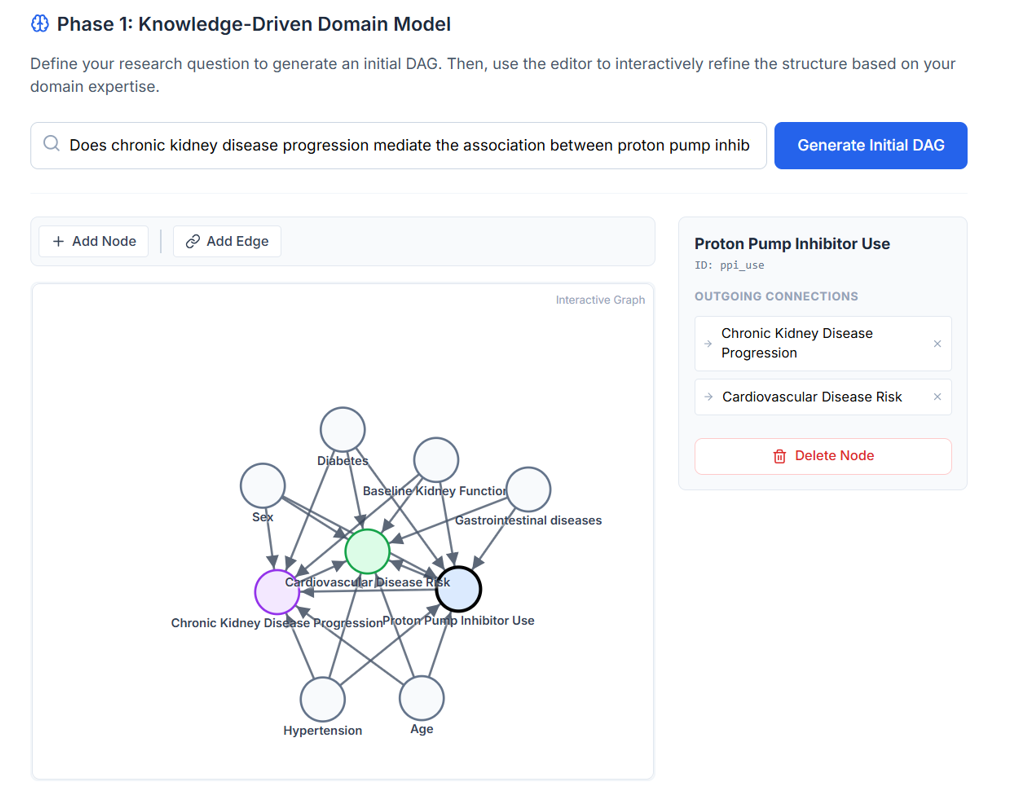
\includegraphics[width=0.75\textwidth]{figures/figure2.png}
  \captionsetup{font=scriptsize}
  \caption{Knowledge-based and expert-refined directed acyclic graph (DAG) for the proof-of-concept case study (Phase 1). In the application, the researcher enters a research question (e.g., ``Does PPI use accelerate CKD progression?'') and the LLM synthesises published literature to generate an initial DAG identifying exposure (PPI use), outcome (cardiovascular disease), mediator (CKD progression), and candidate confounders. Using the interactive graph editor, human experts reviewed the AI-generated structure and applied targeted refinements: CKD progression was explicitly encoded as a mediator on the PPI--cardiovascular pathway, and several candidate confounders (age, sex, diabetes, hypertension, baseline eGFR) were added or repositioned. Nodes are colour-coded by causal role: blue (exposure), green (outcome), purple (mediator), grey (confounder). Solid arrows represent hypothesised direct causal relationships; dashed arrows represent potential confounding pathways. The refined DAG served as the structural basis for event log construction and subsequent process mining in Phase 2.}
  \label{fig:dag}
\end{figure}

\subsection{Target Estimand and Target Trial}

To ensure the causal question is well-defined and distinct from the statistical methodology used to estimate it, the analysis of proton pump inhibitors (PPIs) versus histamine-2 receptor blockers (H2Bs)  is grounded in the target trial emulation framework. Figure~\ref{fig:trial} outlines the hypothetical randomized trial protocol that the observational analysis seeks to emulate.

\begin{figure}[h]
  \centering
  \includegraphics[width=\textwidth]{figures/figure3.png}
  \captionsetup{font=scriptsize}
  \caption{Hypothetical randomized trial protocol derived from the literature-generated DAG.}
  \label{fig:trial}
\end{figure}


\subsection{Process Mining-Derived Disease Trajectories}
In the next phase, the event log was reconstructed directly from the relational database using a targeted SQL extraction query informed by an underlying clinical directed acyclic graph (DAG). The log was generated by performing a UNION operation across the \textit{Lab Results} and \textit{Encounters} tables, joining them with the Patients table to retrieve static case characteristics. To ensure the accuracy of the clinical trajectories, synthetically injected baseline lab values were filtered out by isolating only the tests with values of 60 or below, explicitly defining the "CKD outcomes." The extracted dataset—containing case identifiers, activity types, timestamps, and group assignments—was chronologically sorted. Guided by the knowledge embedded in the conceptual DAG, explicit sequential weights were assigned to each activity type (ranging from 1 for the index drug use to 999 for the study end) to enforce the logical clinical flow. These event logs thus capture the deterministic, longitudinal transitions among drug use, CKD progression, heart disease, and death. 

Process mining discovery techniques were then applied to this sequenced log to generate an empirical process model that reflects the reconstructed clinical trajectories.To generate the empirical process model, a directly-follows graph (DFG) mining approach was implemented to map the chronological sequence of events. The algorithm begins by grouping the reconstructed event log by case identifier and sequentially sorting the events based on their timestamps to reconstruct individual patient trajectories. For each patient trace, the algorithm extracts pair-wise transitions, recording every instance where one clinical activity directly precedes another. These transitions are aggregated across the entire cohort to establish the nodes and the directed edges . To quantify the flow between events, edge strengths are normalized against the maximum transition frequency within the dataset. Additionally, nodes are heuristically classified into clinical roles—such as exposures, mediators, competing risks, and outcomes—based on their specific activity labels. Finally, the algorithm aggregates identical patient pathways to calculate the frequency of distinct process variants, summarizing the most common clinical trajectories observed in the cohort.

These process patterns enabled direct comparison between empirically observed transitions and those implied by the initial literature-informed DAG. Using the Human--AI Governance Panel (Figure~\ref{fig:processmodel}), the tool's suggestion engine systematically contrasted the DFG-derived process model against the knowledge-based DAG and proposed candidate structural refinements, each accompanied by supporting data evidence allowing human experts to adjudicate each proposal individually. 

\begin{figure}[H]
  \centering
  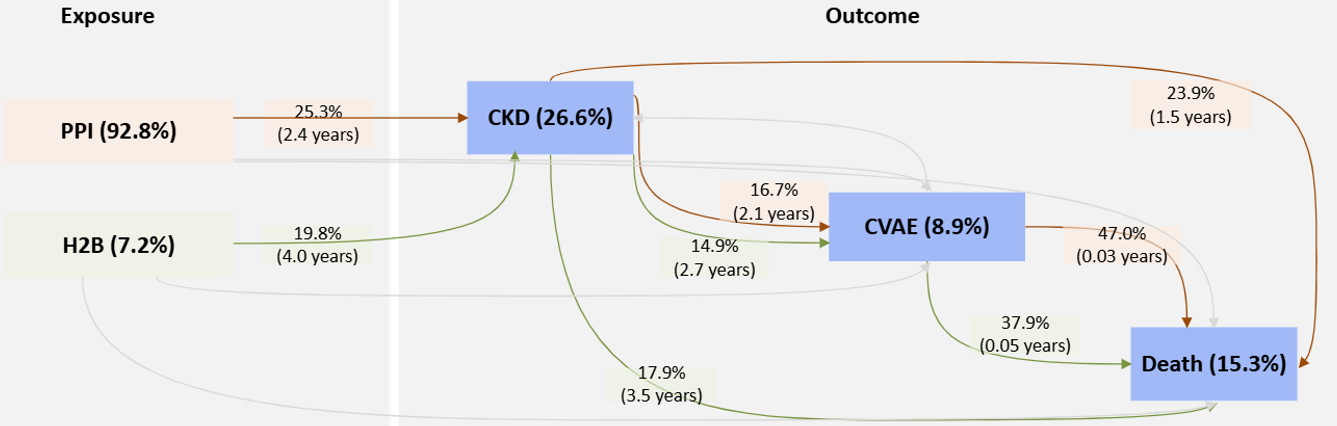
\includegraphics[width=\textwidth]{figures/figure4.png}
  \captionsetup{font=scriptsize}
  \caption{Process model (directly-follows graph) of observed clinical trajectories for PPI and H2B users in the SCREAM cohort (Phase 2, $n = 294{,}734$). The DFG is constructed automatically from uploaded event-log data: the tool parses the CSV, performs data-quality checks (detecting missing values, duplicates, and timestamp inconsistencies), groups events by patient, and computes transition frequencies and median transition times between consecutive events. The node represents the event and displays the relative case frequency (in brackets), which is the proportion of individuals (cases) experiencing the event among all included individuals. The edge (arrow) represents time-ordered sequences of events and displays two statistics: relative-antecedent frequency (risk), which is the proportion of exposure event (antecedent) individuals (cases) directly followed by the target individuals (cases); and median time (in brackets) represents the time from the exposure event to the outcome or competing event, in years. Only statistically significant transitions between PPI and H2B, with a transition risk greater than 10\%, are shown in the indicator.}
  \label{fig:processmodel}
\end{figure}

To illustrate the governance process in practice, the suggestion engine proposed adding a competing-risk node (Death) based on the observed high-frequency mortality transitions from both CKD and CVAE states (confidence: high); this proposal was accepted because competing mortality is biologically expected and methodologically consequential for model specification. Conversely, Figure~\ref{fig:govpanel} shows a proposal to add a direct feedback edge from CVAE to Drug use was rejected as clinically implausible, since medication changes following cardiovascular events reflect clinical management rather than a causal pathway.

\begin{figure}[H]
  \centering
  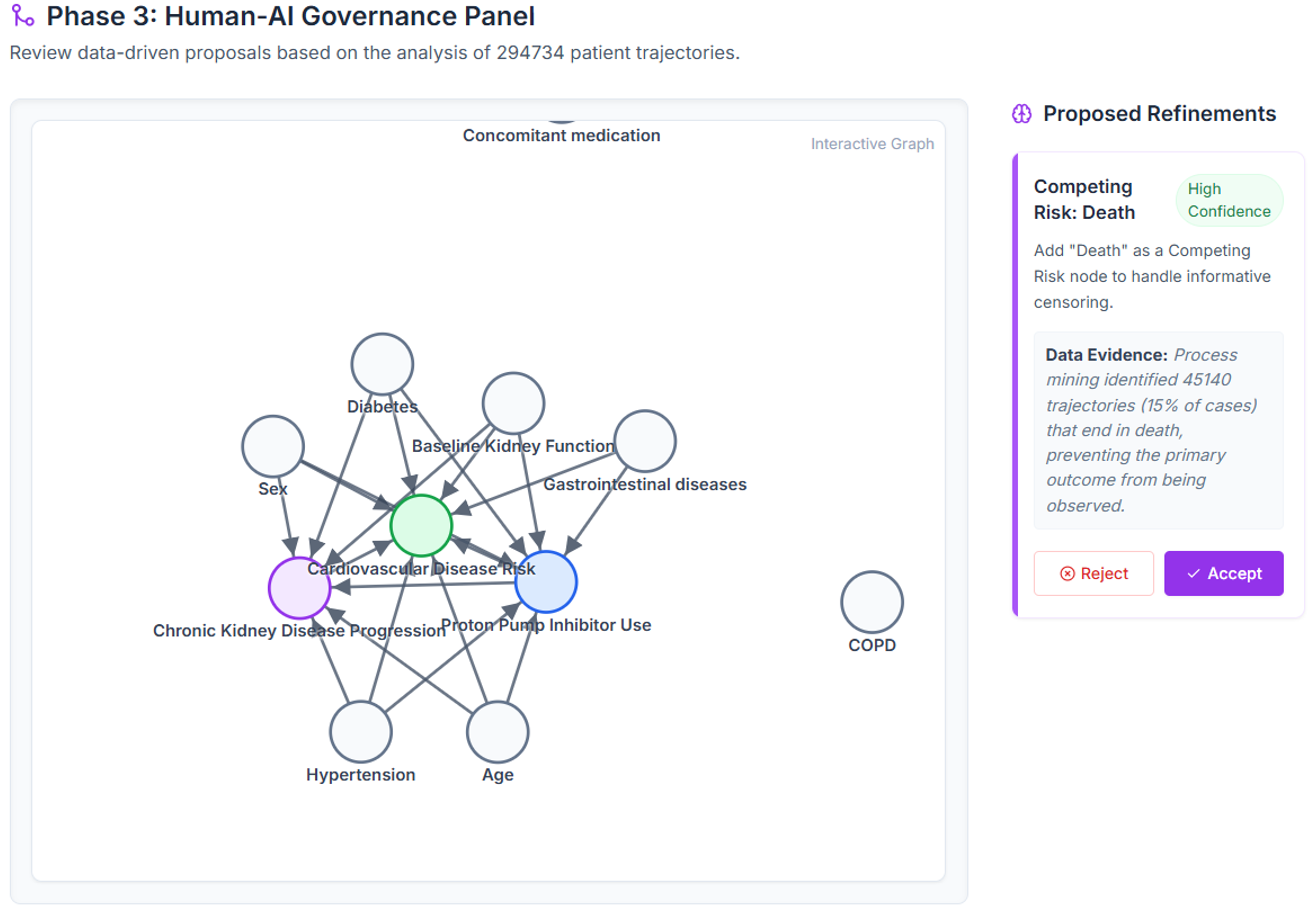
\includegraphics[width=\textwidth]{figures/figure5.png}
  \captionsetup{font=scriptsize}
  \caption{Phase 3 output: the Human--AI Governance Panel for structured DAG refinement. The left panel displays the current DAG as an interactive force-directed graph, colour-coded by causal role (blue = exposure, green = outcome, red = competing risk, purple = mediator, grey = confounder). The right panel presents AI-generated candidate refinements, each showing the proposed structural change (e.g., ``Competing Risk: Death'', ``Mediator: Acute Kidney Injury''), a confidence rating (High/Medium), and the supporting data evidence drawn from the process mining results. The researcher accepts or rejects each proposal individually; accepted changes update the DAG in real time, and a decision log records all adjudications. In this case study, discrepancies flagged by the tool included: (i) the consistently observed CKD$\to$CVAE transition confirming the mediating role of CKD; (ii) the absence of a statistically significant CVAE$\to$CKD transition in PPI versus H2B users; and (iii) high competing mortality rates suggesting the need for competing risk models. Three structural refinements were proposed and accepted following expert biological plausibility review.}
  \label{fig:govpanel}
\end{figure}

\subsection{Data-Driven Refinement of the Causal Model}
The evidence-refined DAG differs from the initial knowledge-based DAG in three key respects, each discovered through the closed-loop process, as it is summarized in Table~\ref{tab:transitions}. First, a competing-risk node (Death) was added, prompted by the high mortality transition rates from both CKD and CVAE states that the initial DAG did not represent. Second, the edge directionality between CKD and CVAE was consistent with the hypothesised direction: the DFG showed consistent CKD-to-CVAE transitions but no significant differential in CVAE-to-CKD transitions between exposure groups. Third, temporal dynamics (median transition times and IQR ranges) were attached to each edge, enabling time-aware model specification. Without the process mining step, the initial knowledge-based DAG would have lacked the competing-risk architecture and the temporal quantification, potentially leading to standard Cox regression rather than the competing-risk and mediation models that the refined DAG warranted. The refined DAG incorporated insights from the process mining results, particularly regarding the temporal ordering and strength of transitions among CKD, CVAE, and death. Notably, in the synthetic data, CKD$\rightarrow$CVAE transitions were frequently observed, and the between-group comparison of CVAE$\rightarrow$CKD transitions did not reach statistical significance. This pattern should not be over-interpreted: a non-significant between-group test does not establish absence of a causal pathway in either direction, and observed transition asymmetry is consistent with --- but does not adjudicate --- a mediating role for CKD. Absent or weakened DFG edges should be treated as hypotheses of non-effect requiring sensitivity analysis, not as evidence of biological non-occurrence. Formal causal mediation analysis, as recommended in Phase 4, would be required to quantify the mediated proportion and test the mediator hypothesis statistically.

\begin{sidewaystable}[p]
\caption{Transition rates and crude rate ratios for process-mining trajectories comparing PPI and H2B users.}
\label{tab:transitions}
\centering
\tiny
\setlength{\tabcolsep}{2.5pt}
\renewcommand{\arraystretch}{1.12}
\begin{tabularx}{\textheight}{@{}>{\raggedright\arraybackslash}p{2.7cm}rrrrrrrrrr@{}}
\toprule
 & \multicolumn{4}{c}{\textbf{PPI}} & \multicolumn{4}{c}{\textbf{H2B}} & \multicolumn{2}{c}{\textbf{PPI vs H2B}} \\
\cmidrule(lr){2-5} \cmidrule(lr){6-9} \cmidrule(l){10-11}
\textbf{Transition} & \textbf{Events} & \textbf{At risk} & \textbf{Risk, \%} & \textbf{Median (IQR), y} & \textbf{Events} & \textbf{At risk} & \textbf{Risk, \%} & \textbf{Median (IQR), y} & \textbf{RR (95\% CI)} & \textbf{$p$} \\
\midrule
\multicolumn{11}{@{}l}{\textit{Key transitions used for DAG refinement}} \\
Medication$\to$CKD & 69,177 & 273,569 & 25.3 & 2.4 (0.7, 5.7) & 4,181 & 21,165 & 19.8 & 4.0 (1.4, 7.7) & 1.28 (1.24, 1.32) & $<$0.001 \\
CKD$\to$CVAE & 12,355 & 73,823 & 16.7 & 2.1 (0.4, 4.7) & 665 & 4,466 & 14.9 & 2.7 (0.6, 5.4) & 1.12 (1.05, 1.21) & 0.002 \\
CKD$\to$Death & 17,659 & 73,823 & 23.9 & 1.1 (0.2, 3.5) & 798 & 4,466 & 17.9 & 1.4 (0.3, 4.3) & 1.34 (1.26, 1.43) & $<$0.001 \\
CVAE$\to$Death & 11,610 & 24,707 & 47.0 & 0.03 (0, 1.2) & 538 & 1,421 & 37.9 & 0.05 (0, 1.8) & 1.24 (1.16, 1.33) & $<$0.001 \\
\addlinespace[2pt]
\multicolumn{11}{@{}l}{\textit{Additional observed transitions}} \\
Medication$\to$CVAE & 12,352 & 273,569 & 4.5 & 2.9 (1.0, 5.9) & 756 & 21,165 & 3.6 & 3.9 (1.6, 7.3) & 1.26 (1.18, 1.36) & $<$0.001 \\
Medication$\to$Death & 13,967 & 273,569 & 5.1 & 1.5 (0.4, 4.1) & 568 & 21,165 & 2.7 & 3.5 (1.3, 6.7) & 1.90 (1.75, 2.07) & $<$0.001 \\
CVAE$\to$CKD & 4,646 & 24,707 & 19.0 & 0.7 (0.1, 2.4) & 285 & 1,421 & 20.1 & 1.4 (0, 1.8) & 0.94 (0.84, 1.04) & 0.238 \\
\bottomrule
\end{tabularx}
\par\smallskip
\noindent\scriptsize\textit{Note.} Risk is calculated as events divided by the number at risk. RR denotes the crude risk ratio comparing PPI with H2B; 95\% confidence intervals were derived using the log method. Median time is reported in years with interquartile range. Statistics were originally published in \citep{chen2025} and are reproduced here to illustrate how process-mining outputs inform DAG refinement.
\end{sidewaystable}

\subsection{AI-Guided Analytical Strategy and Model Configuration}
Using the evidence-refined DAG, the Phase 4 module  analysed the DAG structure, detecting competing-risk nodes, mediator pathways, and confounder sets, and generated analytical recommendations ranked by bias reduction, efficiency, complexity, and clinical interpretability, as shown in Figure~\ref{fig:modelling}. For this case study, the tool identified Fine--Gray competing-risk regression as a candidate strategy for cumulative-incidence estimands, based on the presence of a competing-risk node (Death) in the refined DAG. Cause-specific hazard models would be the appropriate alternative when the target estimand is etiologic transition intensity rather than cumulative incidence; the choice depends on the pre-specified target estimand. The rationale for this choice was explicitly provided, together with model configuration recommendations. In addition, causal mediation analysis was recommended to formally assess the mediating role of CKD progression in the association between PPI use and cardiovascular outcomes. Given the observed imbalance in baseline characteristics between PPI and H2B users, the AI also proposed propensity score--based balancing strategies to improve covariate comparability between groups. Overall, these recommendations were consistent with epidemiological best practices and provided a structured, transparent framework to support researchers in selecting appropriate analytical approaches and model configurations.

\begin{figure}[H]
  \centering
  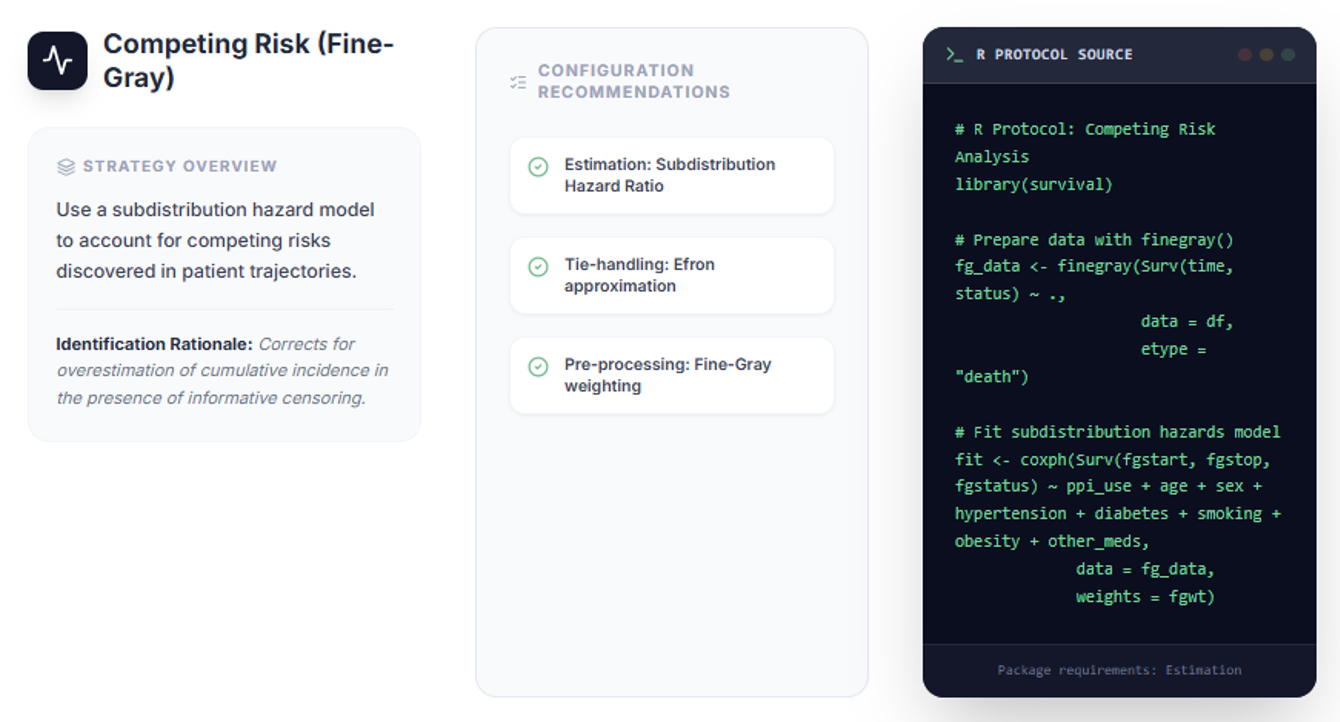
\includegraphics[width=\textwidth]{figures/figure6.png}
  \captionsetup{font=scriptsize}
  \caption{ProcessAI Phase 4 output: Modelling Strategy Summary with analytical recommendations generated from the refined data-driven DAG. The tool analyses the refined DAG structure, detecting competing-risk nodes, mediator pathways, and confounder sets, and recommends appropriate statistical models, each rated across four dimensions (bias reduction, efficiency, complexity, and clinical interpretability) in a comparative summary table. A highlighted primary recommendation identifies the optimal strategy for the observed DAG structure. For this case study, the tool recommended three analytical strategies: (1) Fine--Gray competing risk models to account for high all-cause mortality rates observed in both CKD and CVAE states (see Medication$\to$Death and CKD$\to$Death transitions in Table~\ref{tab:transitions}); (2) formal causal mediation analysis to quantify the proportion of the PPI--cardiovascular association mediated through CKD progression; and (3) propensity score--based covariate balancing to address the observed imbalance in baseline characteristics between PPI and H2B users. Each recommendation included explicit epidemiological rationale and corresponding R code templates. All recommendations were reviewed and accepted by the study team as consistent with established epidemiological best practice.}
  \label{fig:modelling}
\end{figure}

\subsection{Results -- Ground-truth simulation study}

\subsubsection{Calibration}
With the calibrated parameters, the recorded event log approximately reproduced the Table 4 transition-risk pattern, with a worst absolute discrepancy of 0.055 (largest for the H2B S0$\rightarrow$S1 risk) under a pre-specified tolerance of 0.08, and the injected artefacts appeared at the expected frequencies (the reverse CVAE$\rightarrow$CKD coding shift at 0.246/0.245 for PPI/H2B, comparable to Table 4's CVAE$\rightarrow$CKD row). PPI users showed the expected surveillance signature --- shorter CKD detection delay than H2B users at identical latent onset.

\subsubsection{Structural recovery and artefact resistance}
Table~\ref{tab:structural-recovery} reports structural recovery averaged over $M = 500$ replications. The governed configuration (Arm B) recovered all high-support true transitions surfaced by process mining and added the Death competing-risk node in every replication, with perfect edge precision but one missing rare background-mortality edge (recall 0.83); the ungoverned configuration (Arm A) accepted both injected artefacts in every replication, degrading precision. Fig. S2 contrasts the refined graphs: Arm A retains both red artefact edges, whereas Arm B rejects them and adds the Death competing-risk node.

\begin{table}[h]
\caption{Structural recovery at the base cell (mean over $M = 500$; $n = 5{,}000$).}
\label{tab:structural-recovery}
\centering
\footnotesize
\begin{tabularx}{\textwidth}{@{}Ycccccc@{}}
\toprule
\textbf{Arm} & \textbf{Precision} & \textbf{Recall} & \textbf{F1} & \textbf{SHD} & \textbf{Traps accepted} & \textbf{Accepts $\ge 1$ trap} \\
\midrule
A --- ungated proposal-only & 0.71 & 0.83 & 0.77 & 3.00 & 2.00 & 100\% (0.99--1.00) \\
B --- governed (gate) & 1.00 & 0.83 & 0.91 & 1.00 & 0.00 & 0\% (0.00--0.01) \\
C --- oracle & 1.00 & 1.00 & 1.00 & 0.00 & 0.00 & 0\% \\
\bottomrule
\end{tabularx}
\end{table}

The primary contrast was unambiguous: Arm A accepted at least one artefact in 100\% of replications and Arm B in 0\%. The decoy (S2$\rightarrow$S0) was rejected by the activity-type rule (a medication change is administrative, not a disease transition --- the Fig. 5 rationale) and the coding shift (S2$\rightarrow$S1) by the directionality rule (it reverses the CKD$\rightarrow$CVAE order); the ungoverned arm, lacking these rules, accepted both because their directly-follows support ($\approx$0.34 and $\approx$0.18) exceeded the threshold. Recall was 0.83 for both data-driven arms, not 1.0: the rare direct background-mortality edge S0$\rightarrow$S3 (recorded risk $\approx 0.05$) falls below the 10\% discovery threshold and is therefore not surfaced by process mining at this sample size --- a sample-size limitation (Table 2/Table 5) --- though the Death node is nonetheless recovered through the high-mortality S1$\rightarrow$S3 and S2$\rightarrow$S3 transitions.

\subsubsection{Estimand recovery}
Table~\ref{tab:estimand-recovery} reports the exposure log-HR on CKD onset (true value 0.25). Fit to the underlying disease process, the cause-specific Cox model recovered the truth with negligible bias and near-nominal 95\% coverage (mean $\hat{\beta} = 0.250$, 95\% Monte Carlo interval 0.123--0.387), confirming that the model class the framework selects is correct. Fit to the \textit{recorded} times, the estimate was inflated by surveillance bias and its coverage fell below nominal. Naively adjusting for the realised visit count did not repair this --- it over-corrected (collider bias, because visit count is endogenous to follow-up duration); this post-hoc adjustment is a failed comparator, not the recommended model, and its failure is precisely why the framework treats surveillance bias as a \textbf{structural} diagnostic (the monitoring-attenuation check at the gate) rather than a covariate adjustment. The CKD$\rightarrow$CVAE exposure effect, whose true value is zero, was estimated as a small non-significant positive effect on the recorded data, mirroring the manuscript's observation that the between-group CVAE/CKD signal does not reach significance.

\begin{table}[h]
\caption{Estimand recovery for the exposure log-HR (mean over $M = 500$).}
\label{tab:estimand-recovery}
\centering
\footnotesize
\begin{tabularx}{\textwidth}{@{}Yccccc@{}}
\toprule
\textbf{Target} & \textbf{True $\beta^E$} & \textbf{Mean $\hat{\beta}^E$} & \textbf{Bias} & \textbf{RMSE} & \textbf{95\% CI coverage} \\
\midrule
S0$\rightarrow$S1, latent process (estimator validity) & 0.25 & 0.250 & -0.000 & 0.067 & 0.96 \\
S0$\rightarrow$S1, recorded (surveillance-inflated) & 0.25 & 0.327 & +0.077 & 0.105 & 0.83 \\
S0$\rightarrow$S1, post-hoc visit-count adjusted (not recommended) & 0.25 & 0.636 & +0.386 & 0.395 & 0.01 \\
S1$\rightarrow$S2, recorded (true effect null) & 0.00 & 0.180 & +0.180 & 0.273 & 0.91 \\
\bottomrule
\end{tabularx}
\end{table}

The mediated proportion of the PPI$\rightarrow$CVAE effect flowing through CKD, estimated by high-precision g-computation on the known simulator ($n = 50{,}000$), was 0.45 (natural indirect effect 0.007 on a total effect of 0.016 in CVAE cumulative incidence by 10 years), confirming that CKD lies on a genuine --- though partial --- mediating pathway in the DGP.

\subsubsection{Summary}
In this calibrated base-cell stress test, with a known DGP and deliberately injected observation artefacts, the governed loop (Arm B) recovered all high-support true transitions including the competing-risk node and rejected both artefacts in 100\% of replications, whereas the ungoverned configuration (Arm A) accepted at least one artefact in 100\%. The model the framework selects recovers the true cause-specific hazard ratio at near-nominal coverage on the underlying process. The study provides controlled evidence for several Table 5 hazards --- surveillance bias, post-event coding shifts, competing risks, and the sample-size dependence of discovery --- substantiating those future-work claims with evidence rather than assertion; broader generalisation across sample size, monitoring differential, timestamp granularity, confounding strength, and artefact rates is left to the planned sweeps. The headline contrast and estimand recovery are summarised in Fig. S3.

\begin{figure}[H]
  \centering
  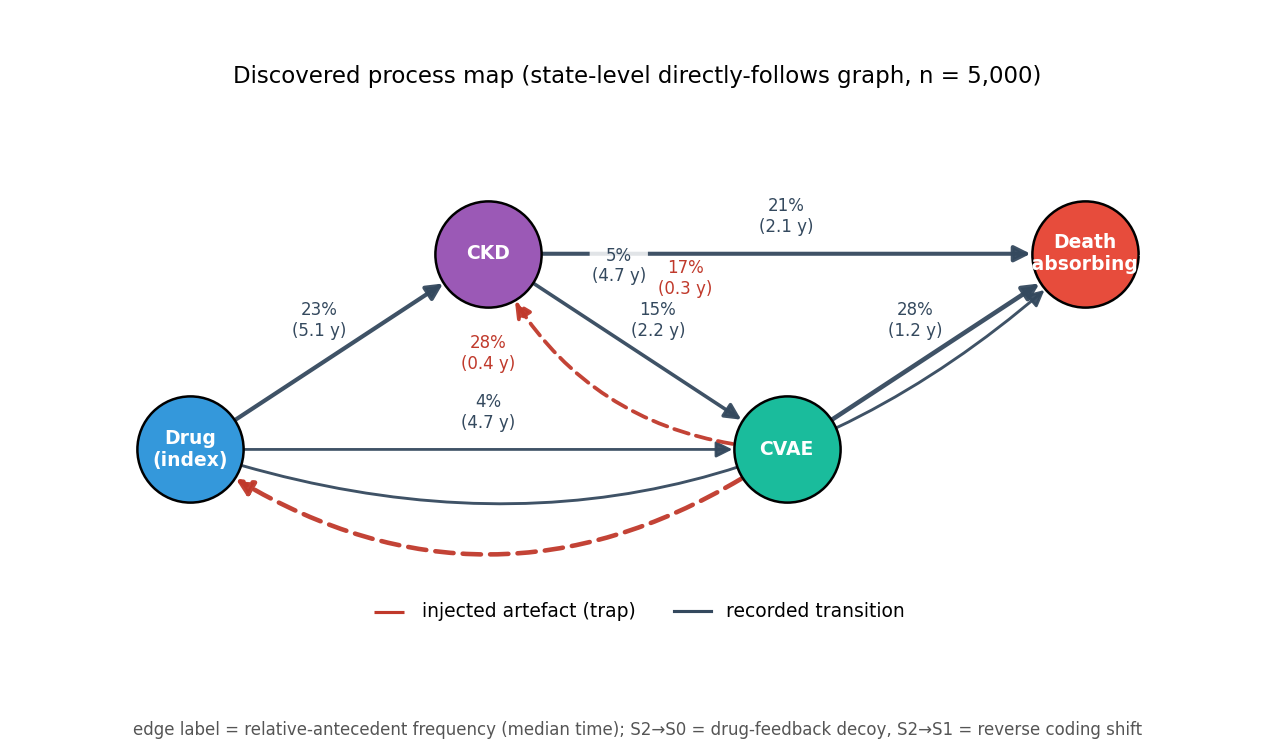
\includegraphics[width=\textwidth]{figures/process_map.png}
  \captionsetup{font=scriptsize}
  \caption{Discovered process map (directly-follows graph) of observed transitions ($n = 5{,}000$). The drug-feedback decoy (S2$\rightarrow$S0) and reverse coding shift (S2$\rightarrow$S1) are shown as red dashed edges.}
  \label{fig:s1}
\end{figure}

\begin{figure}[H]
  \centering
  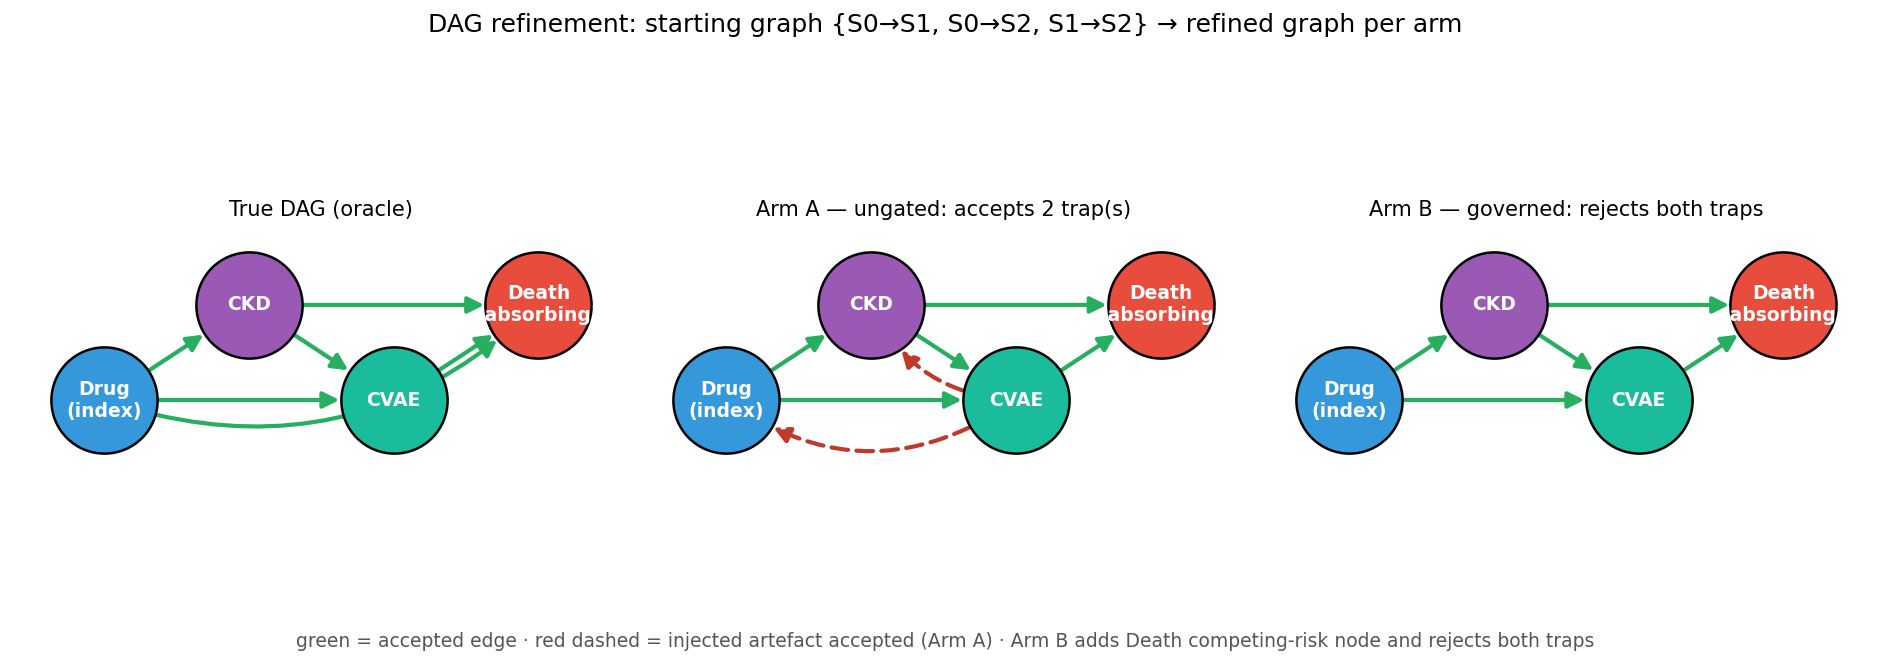
\includegraphics[width=\textwidth]{figures/dag_refinement.png}
  \captionsetup{font=scriptsize}
  \caption{DAG refinement: the true DAG, the Arm A (ungated) refined graph that accepts both artefacts, and the Arm B (governed) refined graph that rejects both and adds the Death competing-risk node.}
  \label{fig:s2}
\end{figure}

\begin{figure}[H]
  \centering
  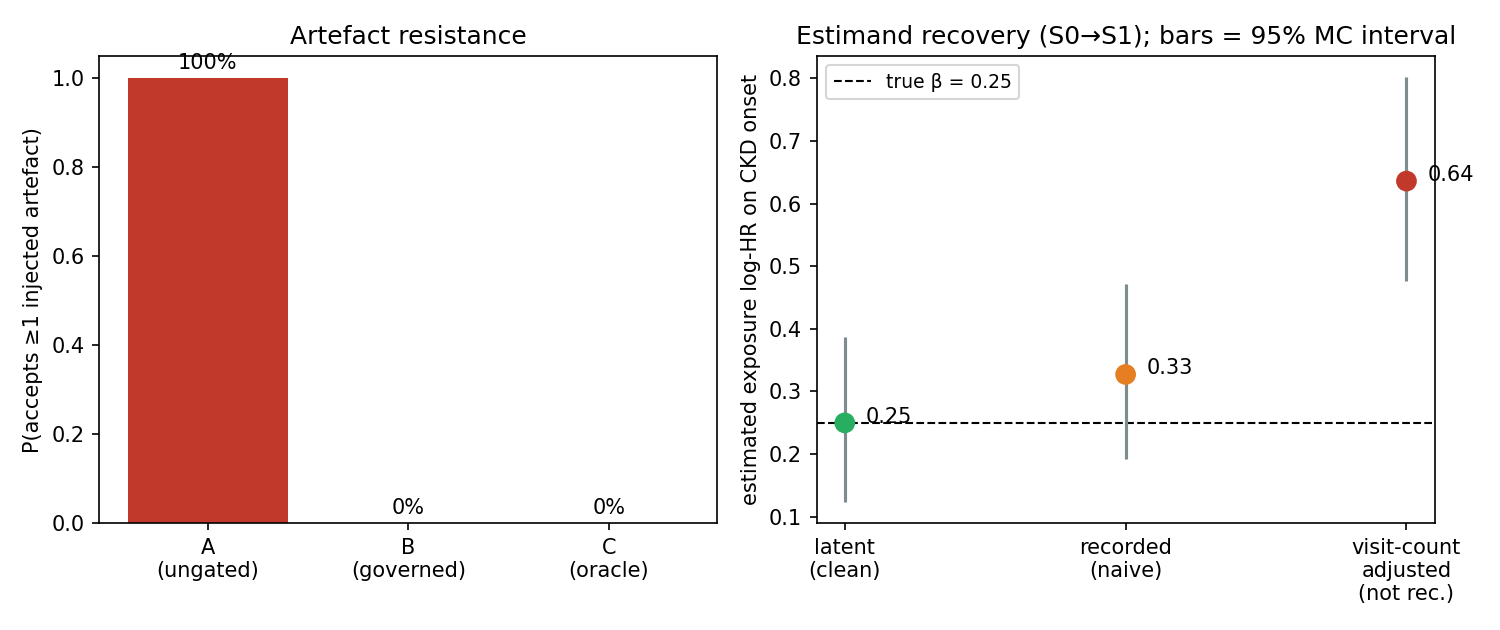
\includegraphics[width=\textwidth]{figures/figure_simulation.png}
  \captionsetup{font=scriptsize}
  \caption{Artefact resistance and estimand recovery (S0$\rightarrow$S1) over $M = 500$ replications. Bars represent 95\% Monte Carlo intervals.}
  \label{fig:s3}
\end{figure}

\section{Discussion}
This study presents a closed-loop human--AI collaboration framework that operationalises causal inference as an iterative, falsifiable, and governance-aware scientific process when using real-world data. Rather than treating DAGs as static representations of prior beliefs or relying solely on automated causal discovery, the framework explicitly positions knowledge-based DAGs as testable hypotheses that can be empirically challenged and refined through longitudinal data. By integrating process mining, expert oversight, and statistical model selection within a single methodological loop, the framework addresses several long-standing limitations in observational health research.

\subsection{Principal Contributions}
The primary contribution of this work lies in reframing the relationship between theory and data in causal epidemiology. Traditional approaches often privilege either expert-driven causal structures, risking misspecification, or data-driven algorithms, risking implausible or clinically uninterpretable results. DAGs provide a transparent method for encoding causal assumptions and identifying adjustment sets for confounding control in observational research \citep{tennant2021}. The closed-loop framework bridges this divide by enabling structured interaction between the two. Empirical temporal patterns discovered through process mining are not interpreted as causal per se; instead, they function as diagnostic signals that appraise the adequacy of existing causal assumptions. This distinction is critical: a directly-follows graph establishes temporal precedence and transition frequency, not causal direction. Process mining evidence can challenge a hypothesised causal structure (e.g., by revealing that an assumed direct pathway operates through an intermediate state) or support it (e.g., by confirming expected temporal ordering), but the causal interpretation of any structural change must be adjudicated by domain experts on grounds of biological plausibility and mechanistic understanding. This distinction, i.e., between diagnostic appraisal and causal proof, preserves the epistemological foundations of causal inference while enabling empirical refinement.

A second key contribution is the formalization of human--AI roles and governance. AI systems are leveraged for literature synthesis, pattern discovery, discrepancy detection, and analytical recommendation, but final causal decisions remain human-led. This design directly addresses concerns about opacity, automation bias, and loss of clinical interpretability that accompany many contemporary AI-driven approaches. The framework therefore advances not only methodological innovation but also responsible AI integration aligned with emerging expectations for transparency and accountability in health research. By pairing AI capabilities with their known limitations, the framework embeds safeguards against hallucination, automation bias, and epistemic overreach.

Third, the framework provides a direct bridge between causal structure and model specification. By translating the evidence-refined DAG into explicit analytical recommendations, the approach reduces a common source of error in applied epidemiology: misalignment between the causal question and the statistical model used to answer it. Notably, the new-user, active-comparator design employed in the tutorial demonstration aligns with the principles of target trial emulation, in which observational analyses are structured to mirror the protocol of a hypothetical randomised trial. The closed-loop framework complements this paradigm by providing a systematic mechanism for specifying and refining the causal structure that the target trial seeks to evaluate.

A critical methodological concern for any iterative refinement approach is the risk of post-hoc rationalization (i.e., fitting causal assumptions to the observed data rather than genuinely testing them). The closed-loop framework addresses this risk through four safeguards. First, each structural refinement must pass a biological plausibility gate adjudicated by domain experts before it is accepted; pattern frequency alone is insufficient justification. Second, decision criteria for accepting or rejecting refinements are pre-specified and documented at each iteration. Third, AI proposes changes and humans decide, with a complete audit trail of what was proposed, what was accepted, and the clinical rationale for each decision. Fourth, the statistical analysis plan is fixed using the refined DAG before any effect estimation is performed, preserving a clear separation between the model refinement phase and the inference phase. Together, these safeguards distinguish the closed-loop approach from undisciplined data mining and align it with established principles of assumption testing in causal epidemiology. 

Because the closed-loop process uses observational data both to refine the DAG and (potentially) to estimate causal effects, confirmatory effect estimation should ideally be performed on (a) an independent dataset, (b) a temporally distinct hold-out period, or (c) a pre-specified split sample reserved before any structural refinements. Where this is infeasible, sensitivity analyses comparing effect estimates under the initial knowledge-based DAG and the evidence-refined DAG should be reported 

\subsection{Insights From the Tutorial Demonstration}

The PPI versus H2B case study illustrates how the closed-loop framework functions in practice. The initial literature-informed DAG hypothesised CKD progression as a mediator between PPI use and cardiovascular adverse events. In the synthetic illustration, process mining of the longitudinal trajectories showed that transitions from CKD to cardiovascular events were consistently observed, whereas reverse transitions (CVAE → CKD) did not differ significantly between exposure groups \citep{chen2025}. This pattern is consistent with prior hypotheses about CKD lying on the PPI–CVAE pathway. It does not adjudicate causal direction, exclude reverse biological effects of CVAE on kidney function, or substitute for formal mediation analysis. Both directions of CKD–CVAE influence are biologically plausible (cardiorenal syndrome), and a non-significant between-group difference is not evidence of absence. Formal causal mediation analysis, as recommended in Phase 4, would be required to quantify the mediated proportion and test the mediator hypothesis statistically.

Importantly, the framework also surfaced clinically relevant competing pathways, particularly the high transition rates to death from both CKD and CVAE states. These illustrative patterns motivated the recommendation to use competing risk models rather than standard survival approaches, illustrating how empirical pattern discovery can provide diagnostic evidence for analytical decisions without undermining causal rigour. That AI-generated recommendations aligned with established epidemiological best practices supports the feasibility of embedding AI assistance within a governed workflow. Prior work on disease progression trajectories using event logs from real-world EHR data supports the utility of process mining for longitudinal pattern discovery in clinical cohorts \citep{chen2024b}.

\subsection{Relation to Existing Methods}

The governance structure is deliberately asymmetrical: AI proposes and humans decide. At each phase, AI capabilities (literature synthesis, pattern discovery, structural comparison, model recommendation) are paired with explicit human responsibilities (event definition, plausibility assessment, causal adjudication, assumption verification). This separation of roles embeds safeguards against automation bias and epistemic overreach while preserving the scalability benefits of AI assistance. 

Traditional question-driven process mining \citep{rojas2017} centres analysis around operational questions formulated by domain experts, while interactive process mining \citep{fernandez2020} emphasises continuous human-in-the-loop engagement. The closed-loop framework extends both paradigms: it operates on a hypothesis-driven causal inference foundation, explicitly formalising prior domain knowledge into testable DAGs, and establishing a governance infrastructure in which human experts retain authority over biological plausibility and causal interpretation.

Unlike automated causal discovery algorithms \citep{pearl2009,glymour2019}, which rely on conditional independence assumptions rarely satisfied in complex healthcare data, the proposed framework does not aim to infer causality from data alone. It embeds temporal pattern discovery within an explicit causal inference framework \citep{montoya2025}, enabling researchers to test and refine causal assumptions against observed data patterns, shifting the focus from descriptive exploration to governed causal refinement.


\subsection{Limitations and Future Work}

A major strength of this framework is its transparency and reproducibility. Each phase produces explicit, inspectable artifacts (DAGs, process models, analytical decisions) that support cumulative scientific learning and stand in contrast to black-box AI systems. However, several limitations warrant consideration. First, the framework does not eliminate residual confounding or data quality limitations inherent in observational data; rather, it aims to make causal assumptions explicit and testable, not infallible. Second, process mining results may be sensitive to event definitions, temporal granularity, and data completeness, underscoring the continued need for expert judgment. Third, while AI tools can scale literature synthesis and pattern recognition, their outputs remain dependent on the quality and scope of underlying knowledge bases. Finally, the current demonstration is based on chronic kidney disease and cardiovascular outcomes within a single healthcare system. While the methodological foundation is robust, broader application across different clinical contexts, diverse populations, and external datasets is needed to fully assess scalability.


The closed-loop framework has important implications for the generation of real-world evidence. By treating causal inference as an iterative learning process, it aligns closely with the realities of longitudinal healthcare data and evolving clinical knowledge. The framework is particularly well suited for studying chronic diseases, multimorbidity, long-term safety, and care trajectories, where causal structures are complex and dynamic. Future research should formalise quantitative criteria for DAG refinement, evaluate inter-rater agreement among experts, benchmark the framework against alternative causal modelling strategies, and explore prospective integration into learning health systems. While the directly-follows graph (DFG) provides valuable empirical evidence regarding temporal succession, relying on process mining to refine causal structures introduces specific challenges as transition patterns observed in healthcare event logs may not accurately reflect latent causal mechanisms due to several confounding factors. Table~\ref{tab:limitations} summarizes the most important topics future work should adress.

\begin{table}[h]
\caption{Future challenges and research gaps.}
\label{tab:limitations}
\centering
\scriptsize
\setlength{\tabcolsep}{4pt}
\renewcommand{\arraystretch}{1.18}
\begin{tabularx}{\textwidth}{@{}>{\raggedright\arraybackslash}p{2.4cm}YYYY@{}}
\toprule
\textbf{Challenge} & \textbf{Description}  \\
\midrule
\textbf{Surveillance Bias} & Differential monitoring intensity between exposure groups can create artifactual transition asymmetries, leading to the false discovery of pathways that merely reflect healthcare utilization \citep{uhl2024evaluating}.   \\
\addlinespace[2pt]
\textbf{Latent Disease Processes} & Process models map the trajectories of recorded clinical events, which often lag behind the latent biological onset of disease \citep{harton2022informative}.  \\
\addlinespace[2pt]
\textbf{Post-Event Coding Shifts} & The occurrence of a severe event may systematically alter subsequent coding practices, such as a reduction in routine CKD monitoring or coding, artificially deflating the frequency of reverse transitions \citep{goldstein2019and}. \\
\addlinespace[2pt]
\textbf{Competing Risks} & The DFG itself can be biased by unadjusted competing risks; the absence of a pathway might simply indicate that patients transition to an absorbing state before the target event can be observed \citep{mollenhoff2024testing}. \\
\addlinespace[2pt]
\textbf{Index-Date Artefacts} & Arbitrary or misaligned index dates can distort the apparent temporal sequence of early events \citep{swerdel2024comparing}. \\
\addlinespace[2pt]
\textbf{Locality of DFGs} & DFGs strictly analyze sequential, event-to-event transitions, which can obscure long-range causal dependencies where an early exposure affects a distant outcome independently of the immediate preceding state \citep{pan2024untapped}.\\
\addlinespace[2pt]
\textbf{Measurement Error} & Misclassification or temporal inaccuracy in nodes can induce spurious edges or mask genuine transitions \citep{goodwin2022timing}. \\
\addlinespace[2pt]
\textbf{Temporal Granularity Limits} & When events are recorded with coarse granularity, true temporal precedence cannot be reliably established, risking the conflation of simultaneous events with sequential pathways \citep{schuster2024analyzing} \\
\bottomrule
\end{tabularx}
\end{table}


\section{Conclusions}

Ultimately, this work operationalizes John Snow's enduring philosophy of empirical falsification within the modern real-world evidence landscape, providing a governed framework for the evidence-informed refinement of knowledge-based causal DAGs. By treating causal assumptions as testable hypotheses rather than static, unyielding structures , our closed-loop workflow leverages process mining as a vital diagnostic tool under a strict regime of structured human adjudication. Through this integrated methodology, initial graphical models are built from prior knowledge, rigorously appraised against longitudinal clinical event sequences, audited via transparent decision provenance logs, and translated into mathematically sound statistical designs. As illustrated by our tutorial validation, this systematic confrontation between conceptual maps and observational trajectories successfully surfaces critical analytical hazards, including hidden mediator pathways and high competing mortality risks. Crucially, this iterative cycle serves to complement—rather than replace—fundamental epidemiological domain expertise, formal identification strategies, and quantitative sensitivity analyses. While future research must benchmark inter-rater reproducibility across independent expert panels and quantify the precise downstream impacts of framework-guided refinements on final effect estimates , the open-source implementation of HealthProcessAI establishes a transparent, governed foundation for bridging the persistent divide between theoretical causal epidemiology and empirical discovery.

\backmatter

\section*{Data Availability Statement}
The developed application tool is available in the project GitHub (https://github.com/eduardo-illueca/healthprocessai-v2), with detailed instructions for deployment. There is also an online demo accesible at https://closed-loop-dag.fly.dev/, including the examples shown in the paper. The synthetic dataset and the script for producing the event log is available at https://github.com/eduardo-illueca/closed-loop-dag/tree/main/dataset.

\section*{Ethics Statement}
The current paper uses only synthetic data for its tutorial demonstration and does not involve human participants.

\section*{Competing Interests}
The authors declare no competing interests.

\section*{Author Contributions}
FA: Methodology development, validation, writing, original draft, project administration, supervision, and resources. KC: Methodology development, formal analysis, data curation, preparation, visualization, review, and editing. FS: Methodology development, supervision, writing, review and editing, funding acquisition, resources. EI: Methodology development, formal analysis, review and editing, supervision. All authors have read and approved the final manuscript.

\section*{Acknowledgments}
This work was supported by EU grant 240038 from EIT Health and SMAILE (Stockholm Medical Artificial Intelligence and Learning Environments) core facility at Karolinska Institute. KC received support from the China Scholarship Council (CSC, No. 201700260176).

\bibliography{sn-bibliography}

\end{document}
